\begin{figure}[!h]
  \begin{center}
    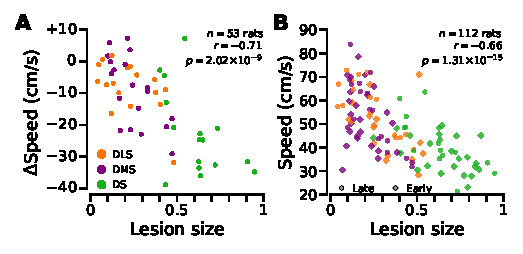
\includegraphics[scale=1]{ch-appendicies/figures/Speed.pdf}
    \caption[Speed-Lesion Size Correlation]
    {\textbf{The impact of the dS lesion on running speed correlates with lesion size.}
    \textbf{(A)} Average change in running speed (speed before lesion$-$speed after lesion) versus lesion size, for all the rats that received a striatal lesion after training (late lesion).
    Running speed was calculated when rats crossed the treadmill from its back region to the reward area.
    All the running speed values obtained across 5 consecutive sessions were averaged to obtain the average running speed before (last 5 sessions before lesion break) and after (sessions \#4 to \#9, relative to lesion break) lesion. 
    \textbf{(B)} Average running speed versus lesion size for all the animals that underwent surgical lesion of the dS.
    This dataset ($n=112$ animals) includes all the animals that underwent striatal lesion (DLS, DMS, DS) after extensive training (Late group, $n=53$, same animals as in panel A), and animals that underwent lesion before training (Early group, $n=59$ animals).
    Speed was computed as in A, except that average was done over session \#25 to \#30, relative to task training onset for the early lesion group.
    }
    \label{fig:appendix:spd}
  \end{center}
\end{figure}